% !TeX spellcheck = fr_FR

% TODO: Replace scan images with clean text where possible

\documentclass[a4paper, 10pt]{report}

\usepackage[french]{babel}
\usepackage[T1]{fontenc}

\usepackage{amsmath, amssymb, amsfonts}

\usepackage{hyperref}
\usepackage{geometry}

\usepackage{xcolor}
\usepackage{graphicx}

\usepackage{fancyhdr}
\usepackage{lastpage}

\usepackage{enumitem}

\geometry{
	a4paper,
	left=25mm,
	right=25mm,
	top=35mm,
	bottom=25mm,
	headsep=5mm,
	headheight=20mm,
}

\definecolor{solution}{HTML}{E5E4E2}
\providecommand{\abs}[1]{\lvert#1\rvert}
\providecommand{\norm}[1]{\lVert#1\rVert}

\begin{document}
	
	\renewcommand{\headrule}{%
		\vspace{-4pt}\hrulefill
		\raisebox{-6.8pt}{\ 
\includegraphics[height=5mm]{../../icon.png}}
		\hrulefill
	}	
	\pagestyle{fancy}
	\fancyhf{}
	
	\fancyhead[L]{\small \slshape Automne 2024}
	\fancyhead[C]{\Large \bfseries Logique et Théorie des Ensembles\\
		Série 08-B}
	\fancyhead[R]{\small Buff Mathias}
	\fancyfoot[L]{
		\small Source files available at:
		\href{https://github.com/MathiasBuff/bsc-math}
		{github.com/MathiasBuff/bsc-math}
	}
	\fancyfoot[R]{
		\small Page \thepage
		\hspace{1pt} /
		\pageref*{LastPage}
	}
	
	
	\noindent
	\textbf{Exercice 1.} Trouver les bornes supérieures et inférieures
	dans $\mathbb{R}$ des ensembles suivants.\\
	(pour $a, b \in \mathbb{R},
	[a, b] = \{x \in \mathbb{R} : a \leq x \leq b\},
	[a, b) = \{x \in \mathbb{R} : a \leq x < b\},
	(a, b] = \{x \in \mathbb{R} : a < x \leq b\}, \text{ et }
	(a, b) = \{x \in \mathbb{R} : a < x < b\}$).
	Préciser lorsque ce sont des maximums et minimums.
	Vous justifierez toutes les réponses.
	\begin{enumerate}[label=\arabic*.]
		\item $[2, 3)$
		\item $[2, 3]$
		\item $(2, 3)$
		\item $(2, 3]$
		\item $[-2, 2] \cup (5, 8)$
		\item $[0,1] + [-3, 7] = \{x + y : x \in [0,1], y \in [-3,7]\}$
		\item $\{\frac{1}{n} : n \in \mathbb{N}^*\}$
		\item $\{x^2 : x \in [-1, 4)\}$
		\item $\{4 + \frac{1 + (-1)^n}{n} : n \in \mathbb{N}^*\}$
	\end{enumerate}
	
	\colorbox{solution}{\begin{minipage}{0.9\textwidth}
		Montrons que l'infimum et le supremum d'un intervalle sont les
		bords de cet intervalle.\\
		
		Soit $[a, b] \subset \mathbb{R}$ un intervalle (preuve similaire
		pour $(a, b], [a, b), (a, b)$).\\
		Par définition, $\forall x \in [a, b], a \leq x \leq b$, donc
		$a$ est un minorant et $b$ un majorant de $[a, b]$.\\
		
		Soit $\varepsilon > 0$. Supposons qu'il existe $M$, majorant de
		$[a, b]$ tel que $M = b - \varepsilon$. Soit alors 
		$x := \frac{b+M}{2}$, nous avons que $x > M$ et $x < b$ donc
		$x \in [a, b]$. Alors $M$ ne peut pas être un majorant de $[a, b]$
		et on en déduit que $b$ est le supremum de $[a, b]$.\\
		
		Par le même raisonnement, on peur montrer que $a$ est l'infimum de
		$[a, b]$.\\
		
		\begin{enumerate}[label=\arabic*.]
			\item $\inf[2, 3) = \min[2, 3) = 2, \quad
				\sup[2, 3) = 3, \quad [2, 3)$ n'a pas de maximum
			%
			\item $\inf[2, 3] = \min[2, 3] = 2, \quad
				\sup[2, 3] = \max[2, 3] = 3$
			%
			\item $\inf(2, 3)  = 2,\quad
				\sup(2, 3) = 3, \quad (2, 3)$ n'a ni minimum ni maximum 
			%
			\item $\inf(2, 3] = 2, \quad
				\sup(2, 3] = \max(2, 3] = 3, \quad (2, 3]$ n'a pas de mimimum
			%
			\item $\inf[-2, 2] \cup (5, 8) = \min{\inf[-2, 2], \inf(5, 8)}
				= -2$ et c'est un minimum\\
			$\sup[-2, 2] \cup (5, 8) = \min{\sup[-2, 2], \sup(5, 8)}
				= 8$ et ce n'est pas un maximum
			%
			\item $\inf\{x + y : x \in [0,1], y \in [-3,7]\} = \inf[-3,8]
				= -3$ et c'est un minimum\\
			$\sup\{x + y : x \in [0,1], y \in [-3,7]\} = \sup[-3,8]
				= 8$ et c'est un maximum
		\end{enumerate}
		
		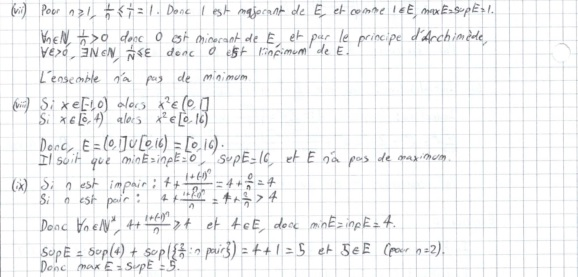
\includegraphics{ex01.jpg}
	\end{minipage}}

	\newpage
	
	\fancyhf{}
	\renewcommand{\headrule}
	{\rule{\textwidth}{0pt}}
	\fancyfoot[R]{
		\small Page \thepage
		\hspace{1pt} /
		\pageref*{LastPage}
	}
	
	\vspace{5mm}
	\noindent
	\textbf{Exercice 2.} (Relation d'ordre totale ou partielle, élément
	maximal) Une relation d'ordre $\leq$ est dite \textit{totale} si 
	$\forall x, y \in E, x \leq y$ ou $y \leq x$, sinon la relation
	d'ordre est dite \textit{partielle}.\\
	Soit $F$ une partie de $E$.
	\begin{enumerate}[label=\arabic*.]
		\item Dire (en justifiant) si les relations d'ordre suivantes sont
		partielles ou totales :
		\begin{enumerate}[label=(\alph*)]
			\item L'inclusion sur $E$
			\item La divisibilité sur $\mathbb{N}$
			\item L'ordre usuel sur $\mathbb{R} : x \leq y$ ssi $y-x \geq 0$
			\item L'ordre lexicographique sur $\mathbb{R}^2$ défini par
			$(x, y)\mathcal{R}(a, b)$ ssi $x < a$ ou $x = a$ et $ y \leq b$
		\end{enumerate}
		\item Un élément $m$ est un \textit{élément minimal} de $F$ si
		$m \in F$ et $\forall x \in F, [m \geq x \implies x = m]$.\\
		Montrer qu'un minorant de $F$ qui est dans $F$ est un élément
		minimal.
		\item Quels sont les éléments minimaux de
		$\mathbb{N} \setminus \{0\}$ pour la divisibilité sur $\mathbb{N}$ ?
		Même question avec $\mathbb{N} \setminus \{0, 1\}$. Montrer qu'un
		élément minimal n'est pas forcément un minorant.
		\item Montrer que si l'ordre est total, alors il existe au plus un
		élément minimal pour $F$.
	\end{enumerate}
	
	\colorbox{solution}{\begin{minipage}{0.9\textwidth}
		\begin{enumerate}[label=\arabic*.]
			\item 
			\begin{enumerate}[label=(\alph*)]
				\item partielle : Soient $F, G \in E$ t.q. $G = E \setminus F$.
				Alors $F \not \subset G$ et $G \not \subset F$
				\item partielle : 2 ne divise pas 3 et 3 ne divise pas 2.
				\item totale : Ou bien $y - x \geq 0$, alors $x \leq y$,
				ou bien $y - x < 0$, alors $y < x$ donc $y \leq x$.
				\item totale : \begin{itemize}[label=-]
					\item Si $x < a$ alors $(x, y)\mathcal{R}(a, b)$
					\item Si $a < x$ alors $(a, b)\mathcal{R}(x, y)$
					\item Si $x = a$ et $y \leq b$ alors $(x, y)\mathcal{R}(a, b)$
					\item Si $x = a$ et $b \leq y$ alors $(a, b)\mathcal{R}(x, y)$
				\end{itemize}
			\end{enumerate}
			\item Par définition d'un minorant : $\forall x \in F, x \geq m$.
			Donc, si $x \in F \leq m$ alors $x = m$, et si $m \in F$ c'est donc
			un élément minimal. 
			\item L'élément minimal de $\mathbb{N}\setminus\{0\}$ pour la
			divisibilité sur $\mathbb{N}$ est 1, car 1 divise tous les éléments
			de cet ensemble, et son seul diviseur est lui-même.\\
			Les éléments minimaux de $\mathbb{N}\setminus\{0, 1\}$ pour la
			divisibilité sur $\mathbb{N}$ sont les nombres premiers, car sur
			cet ensemble ils n'ont qu'eux-mêmes comme diviseur.\\
			Il suit directement du deuxième exemple qu'un élément minimal n'est
			pas forcément un minorant.
			\item Supposons $m$ et $m'$ deux éléments minimaux de $F$ selon une
			relation d'ordre totale.
		\end{enumerate}
	\end{minipage}}
	
	
	\vspace{5mm}	
	\noindent
	\textbf{Exercice 3.} Soit $A$ un sous-ensemble borné non vide de 
	$\mathbb{R}$. Soit $B = \{\abs{x-y}, x \in A \text{ et } y \in A\}$.\\
	Montrer que \[\sup B = \sup A - \inf A\]
	
	\colorbox{solution}{\begin{minipage}{0.9\textwidth}
		Sans perte de généralité, supposons $x > y$. Alors, pour
		$x, y \in A$,\\
		$\abs{x-y} = x - y \leq \sup A - y \leq \sup A - \inf A.$
		Donc $\sup A - \inf A$ est un majorant de $B$ (*)
		
		Soit $m < \sup A - \inf A$ de sorte que
		$m = \abs{s - \inf A}, s \in A < \sup A$.
		Définissons $\delta = \sup A - s$. Alors, $\abs{s - \inf A} =
			\abs{(\sup A - \frac{\delta}{2}) - (\inf A + \frac{\delta}{2})}$
		et comme
		$(\sup A - \frac{\delta}{2}), (\inf A + \frac{\delta}{2}) \in A$,
		alors $\abs{s - \inf A} = m \in B$.\\
		On déduit donc que $\sup A - \inf A \leq \sup B$ (**).
		
		Par (*) et (**), il est montré que $\sup B = \sup A - \inf A$
	\end{minipage}}
	
	\vspace{5mm}
	\noindent
	\textbf{Exercice 4.} Montrer que $\{x \in \mathbb{Q}, x^2 \leq 2\}$
	ne possède pas de supremum dans $\mathbb{Q}$.
	
	\colorbox{solution}{\begin{minipage}{0.9\textwidth}
		\underline{Par l'absurde :}\\
		Supposons que le supremum de $\{x \in \mathbb{Q}, x^2 \leq 2\}$
		existe, et notons-le $S$. Puisque $\mathbb{Q}$ et
		$\mathbb{R} \setminus \mathbb{Q}$ sont denses dans $\mathbb{R}$,
		\[\forall x \in \mathbb{Q}\cap[-\sqrt{2}, \sqrt{2}],
		\exists \varepsilon > 0 \text{ t.q. } S - \varepsilon > x\]
		Alors, $S - \varepsilon < S$ est un majorant de
		$\{x \in \mathbb{Q}, x^2 \leq 2\}$, ce qui contredit la
		supposition que $S$ est le supremum de cet ensemble.
	\end{minipage}}
	
\end{document}
